 \chapter{MC-SBD-STM Results}
%todo: change impurities to defects, defects include impurities and vacancies. 
In this chapter, we present the results from the \ac{MC-SBD} on the synthetic data. We first introduce a synthetic QPI-STM data generation process, build a corresponding system of metrics, and evaluate the performance of the algorithm on a wide range of synthetic data to evaluate the robustness of the algorithm. 

\section{MT-SBD-STM Result on synthetic data}
Evaluating the algorithm's performance on synthetic data is essential, as real experimental data typically lacks access to the ground truth for both the kernel and the activation. To ensure meaningful evaluation, the synthetic datasets must be carefully designed to reflect the physical data generation process observed in experiments. In this section, we demonstrate that the algorithm performs robustly across a wide range of parameter settings. We do so by introducing a simulation method informed by experimental conditions, developing metrics that evaluate the algorithm from three complementary perspectives, and presenting results spanning various regions of the parameter space. Finally, we discuss the scenarios in which the algorithm fails and explore the possible causes.

\subsection{Synthetic Data Generation Process}
The synthetic data generation process follow closely with the convolutional model of QPI-STM that we established in Ch. 5. Mathematically, the synthetic data $Y(\omega)$ is generated via:
\begin{equation}
	Y(\omega) = \sum_i^s ( A_i(\omega) * X_i) + \beta. 
\end{equation} 

%A real STM grid map samples from a continuously varying Local density of states. However, due to the discrete nature of computer simulation, we need to make modifications and even compromises in designing the data generation process. 

In practice, there are 4 parameters that dictates $Y(\omega)$, they are:
\begin{itemize}
	\item Signal to Noise Ratio ($SNR$): the variance ratio between the noiseless kernel and the noise. This influence $\beta$ and $A_i(\omega)$, we will elaborate the latter influence later. 
	\item Observation lattice size ($N_{obs}$): total number of lattice sites per side within the grid map, ie, the grid consists of $N_{obs}*N_{obs}$ lattice sites. This dictates the physical size of the grid map. 
	\item Linear observation resolution ($p$): number of pixels per lattice site, this is enforced to be an integer due to the discrete nature of simulation. 
	\item defect density($\rho_i$): number of defect i per lattice site. Practically, it is equivalent to the probability of a lattice site to host defect i, a formulation according to the statistical framework of defect we established in Ch. 4.
\end{itemize}
\begin{figure}
	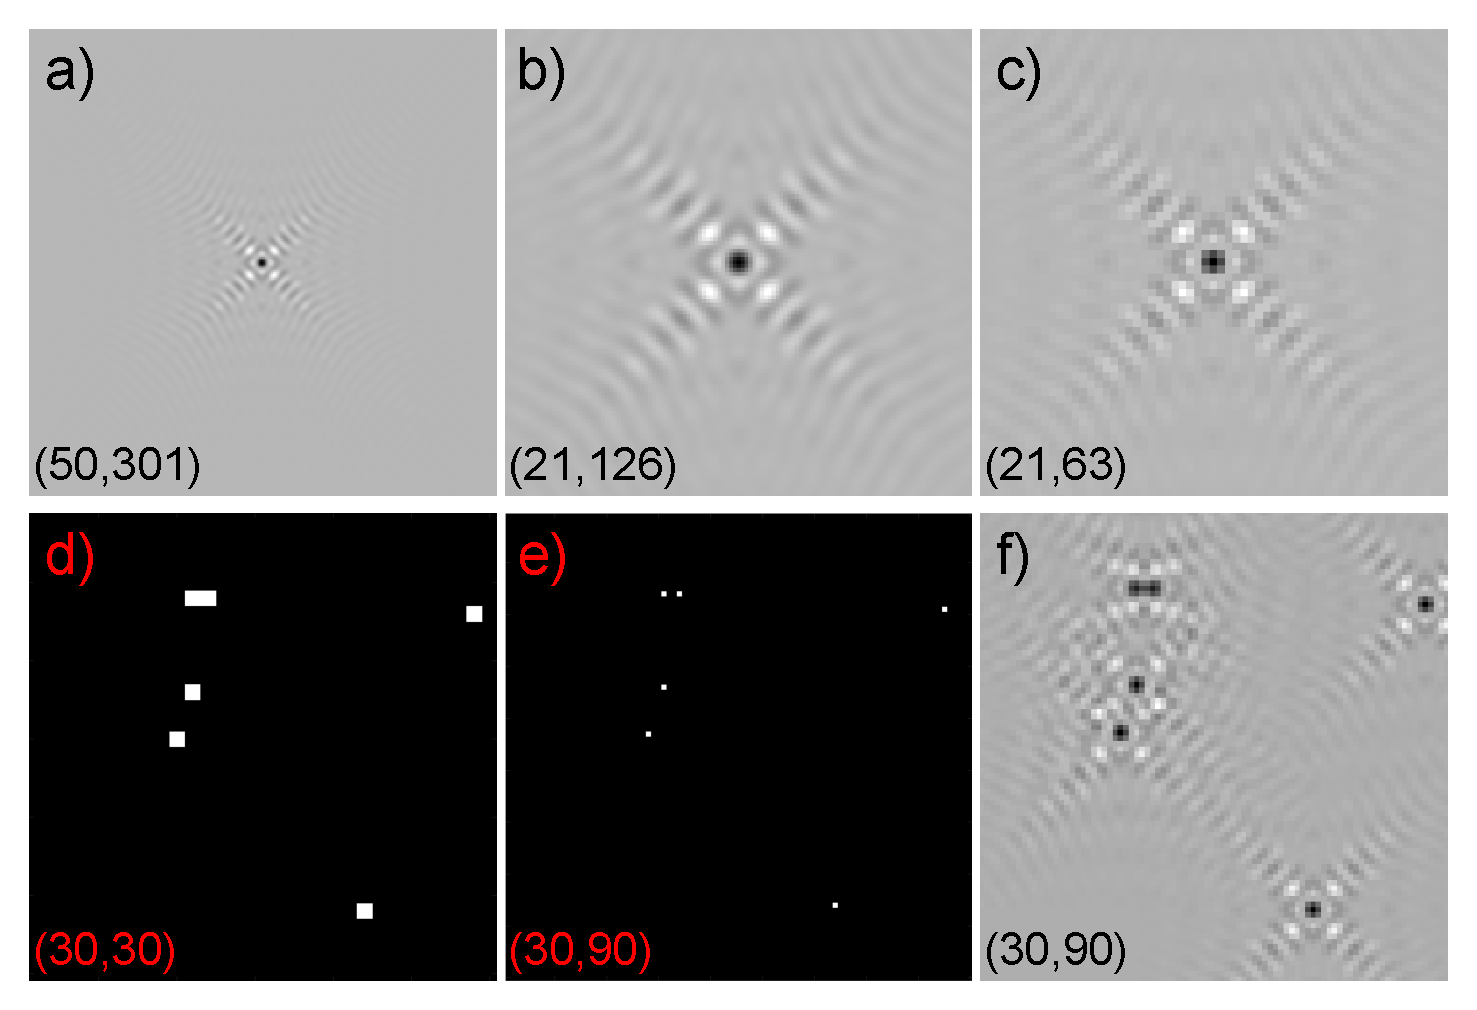
\includegraphics[width= \textwidth]{Ch7_synGen.pdf} 
	\centering
	\caption[\textbf{Illustration of the synthetic data generation pipeline}]{\textbf{Illustration of the synthetic data generation pipeline}. The pair of numbers in the bottom left corner of each subplot reads: (number of lattice sites, number of pixels) per side. Starting from a simulated \ac{LDOS} based on a tight-binding model, we select an energy slice and generate a) with large spatial coverage of 50 lattices and dense sampling (6 pixels per site). A signal-to-noise ratio ($SNR$) is then applied, and the part of signals that was buried under the noise is truncated to get b) \ref{fig:ch7_kernel_size}, mimicking the finite extent of observable \ac{QPI} patterns. Image (c) is obtained by downsampling (b) to simulate the discrete sampling process of \ac{STM}, yielding the ground truth kernel $A^{gt}_i$. The initial activation map d) is generated given the observation lattice size($N_{obs}$) and the defect density($\rho_i$), where each activation site on a lattice site. Then we upsize d) by the linear observation resolution($p$), $p=3$ in this case, and get the ground truth activation map $X^{gt}_i$, shown in (e). A 2D linear convolution between $A^{gt}_i$ and $X^{gt}_i$ produces the component observation $Y^{gt}_i$, which are summed across all $i$ to form the final ground truth observation $Y^{gt}$ f).}
	\label{fig:ch7syn}
\end{figure}

The step by step data generation process is illustrated in Fig. \ref{fig:ch7syn}. It is worth noting that we have a pair of numbers in the bottom-left corner of each subplot. Every pair indicates the $(N_{obs}, N_{obs}*p)$ of this image. We first take the simulated \ac{LDOS} on the tight-binding model we built in Ch.4 and pick an energy slice. We generate the image in Fig. \ref{fig:ch7syn} a) with large $N_{obs}$ and dense pixels. Then we choose an a SNR-ratio $SNR$ and apply it onto the image in Fig. \ref{fig:ch7syn} a), due to the decaying nature of the \ac{QPI} pattern. We can draw an cutoff location where the signals are buried in the noise, as illustrated in Fig. \ref{fig:ch7_kernel_size}. This process gives us b), a truncated version of a) with noise added. a) and b) mimic the underlying \ac{LDOS} on the surface of the specimen that \ac{STM} samples from. In real experiments, this sampling process turns the initially continuous \ac{LDOS} to a discrete grid map. Here, we model this processing through down sampling an initially dense grid($p=6$) b) with a smaller linear observation resolution $p=3$ and get c), our ground truth kernel $A^{gt}_i$. Note that the down sampling only changes the pixel size, but keeps the spatial lattice size unchanged. The activation map is first generated in the lattice grid, as the impurities mostly sit on the lattice sites. Then we resize the activation map to match the linear resolution of the kernel and get e), our ground truth activation map $X^{gt}_i$. Finally, we apply 2D linear convolution to $A^{gt}$ and $X^{gt}$ to get the ground truth observation for kernel $i$: $Y^{gt}_i$. We then repeat this process and composite different observations to construct the final observation $Y^{gt}= \sum_iY^{gt}_i$. 

\begin{figure}
	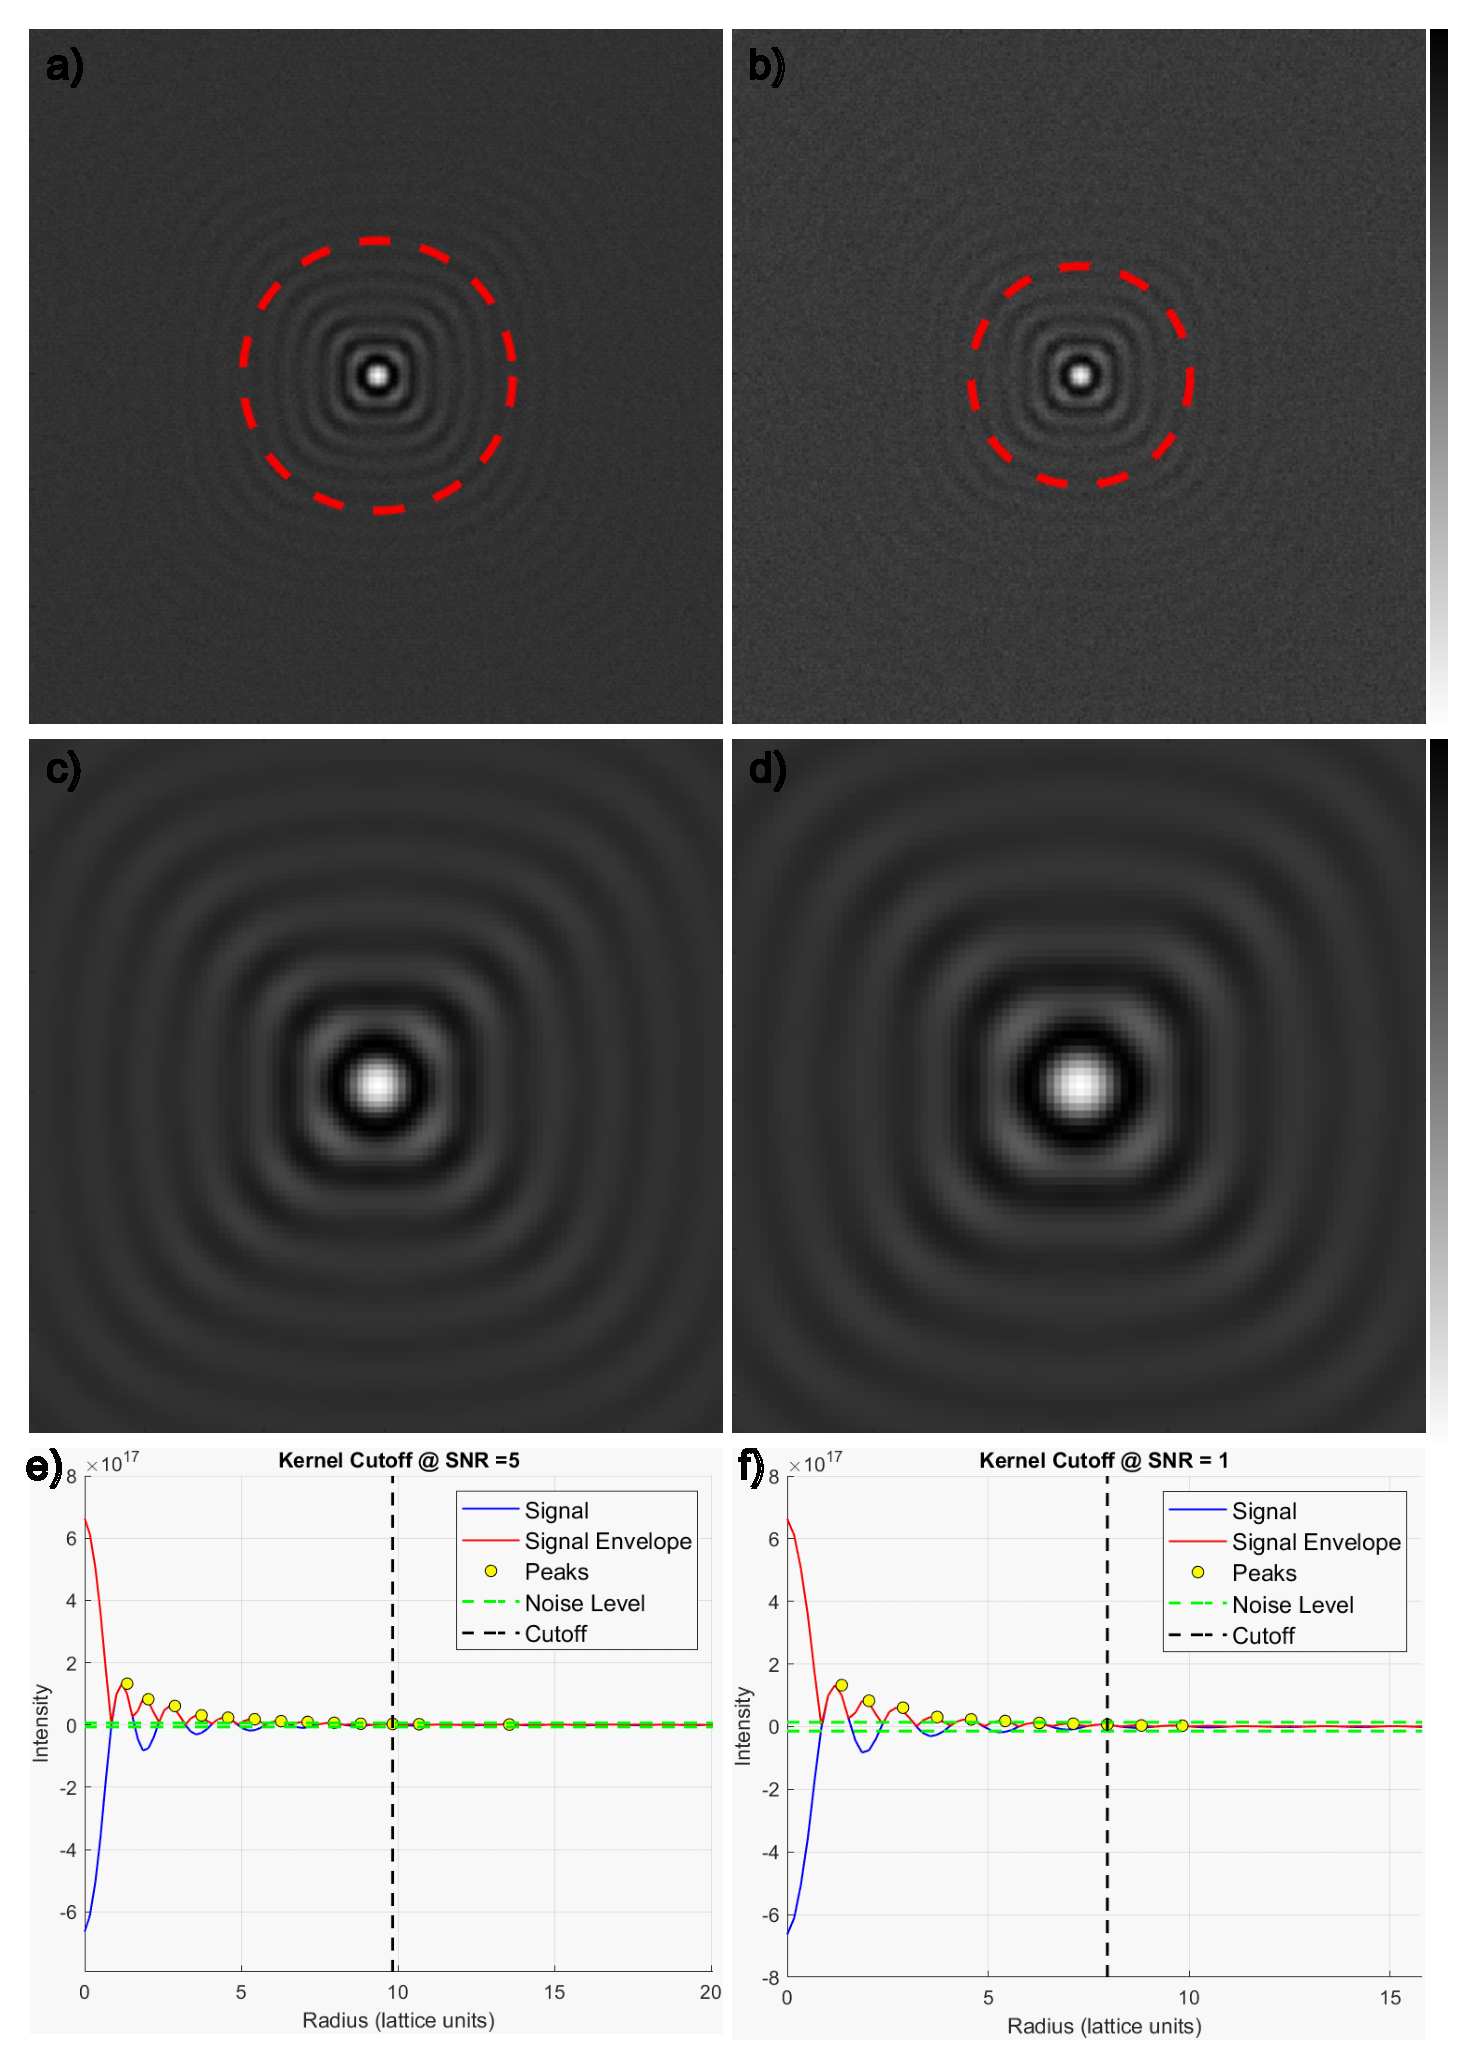
\includegraphics[width= 0.9\textwidth]{Ch7_kernel_size.pdf} 
	\centering
	\caption[\textbf{Kernel truncation according to the noise level}]{\textbf{Kernel truncation according to the noise level}. a), b): the same kernel with different noise level, where the red dotted circle indicates the radial threshold at which the signal drops below the noise. The intensity comparison can be seen in e) and f). The truncated kernel is presented in c) and d).}
	\label{fig:ch7_kernel_size}
\end{figure}

Our simulation approach improves on two key limitations of the original method. First, in the original synthetic data generation workflow proposed by Cheung et al., the kernel was generated by simply selecting a target size and applying the matlab function \textit{imresize} to a large single-defect QPI simulation. This process arbitrarily rescales the entire QPI pattern without considering how far the signal meaningfully extends, leading to unphysical distortion of spatial features. In contrast, our method determines the kernel size based on where the QPI signal becomes indistinguishable from noise, with a defined SNR threshold. This ensures the kernel reflects the true spatial extent of the physically meaningful signal. Second, Cheung et al. placed impurities on a binary pixel grid without regard to the underlying lattice, allowing the impurities to appear off-site—a simplification that breaks down in most materials where defects are confined to lattice points. Our method instead defines the activation map on the actual lattice grid and ensures defects are positioned only at valid lattice sites. These two improvements—grounding the kernel in real signal decay and enforcing lattice-consistent activation—make our simulated data more faithful to experimental conditions and more reliable for algorithm benchmarking.

We now show some examples of the synthetic data generated to give some taste to the readers about how we model datasets in different regimes. As illustrated in Fig. \ref{fig:synexample}, we first plot a reference observation $Y_a$ in a), with 2 different types of defects, $SNR = 5$, $N_{obs}=50$, linear resolution $p = 3$, density of individual type $\rho_i = 0.2 \%$. We can tune the density of individual defect type by changing $\rho_i$, an example is given in b), with $\rho_i$ doubled and other parameters unchanged. We can also tune the spatial resolution of the scan by changing the linear resolution $p$. In c), we present a case where $p$ is doubled, modeling a case where we have a more fine-grained grid map. Lastly, we can expand the physical coverage of the scan by modifying $N_{obs}$. Here, we doubled the $N_{obs}$ and plot the $Y_d$ in d). With these parameters, we can create a parameter space that covers a wide range of different datasets and then test the robustness of our algorithm. Before we do that, we first need to build a metric system that measures the goodness of reconstruction between the algorithm output and the ground truth data. 

\begin{figure}
	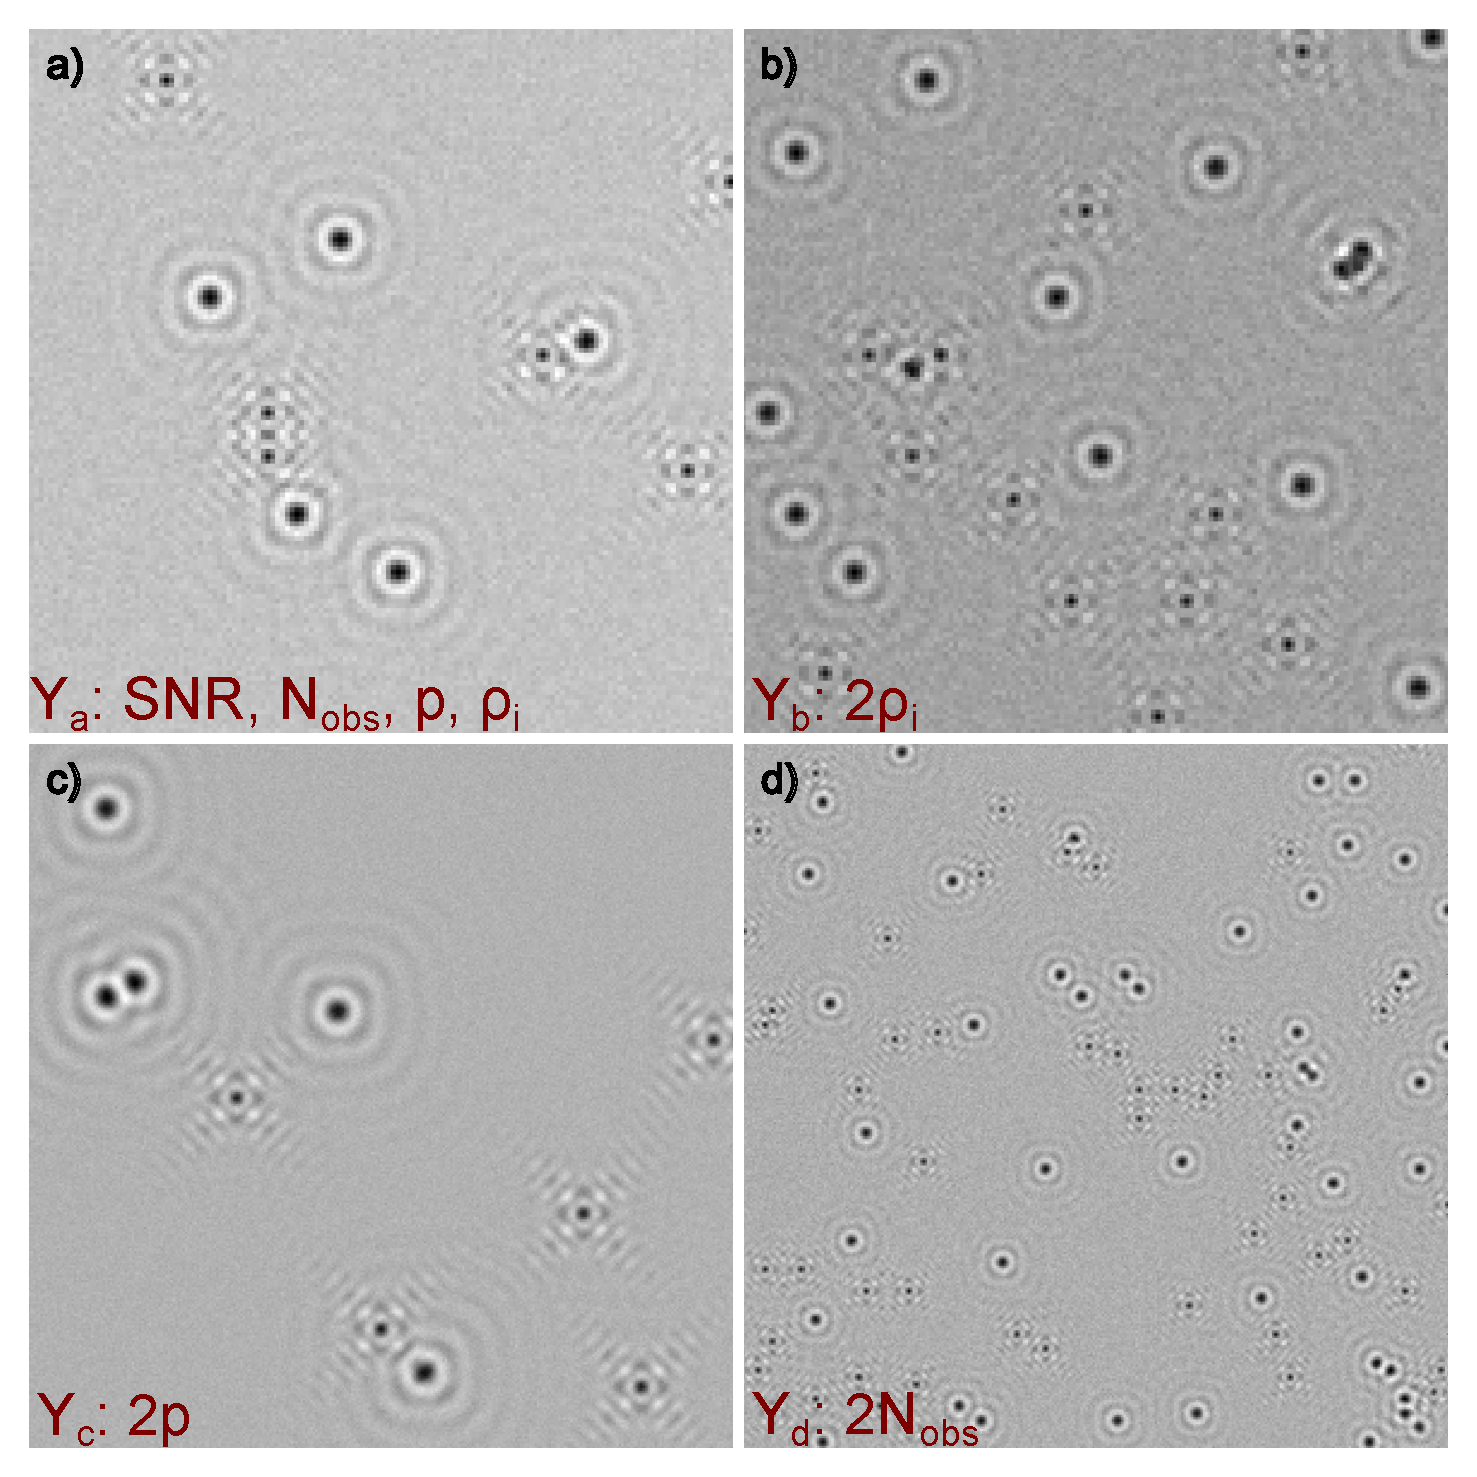
\includegraphics[width= \textwidth]{synGenExamples.pdf} 
	\centering
	\caption[\textbf{Examples of synthetic observations generated by varying key parameters in the simulation pipeline}]{\textbf{Examples of synthetic observations generated by varying key parameters in the simulation pipeline}. (a) Reference observation $Y_a$ with two defect types, $SNR = 5$, $N_{obs}=50$, linear resolution $p=3$, defect density $\rho_i=0.2\%$. (b) Increased defect density ($\rho_i$ doubled) while keeping other parameters fixed. (c) Higher spatial resolution achieved by doubling $p$, resulting in a finer grid. (d) Expanded field of view by doubling $N_{obs}$.}
	\label{fig:synexample}
\end{figure}

\section{MT-SBD-STM Metric system}
The MT-SBD metric system consists of four metrics. They are \textbf{Kernel Similarity(\textit{KS})}, \textbf{Activation Similarity(\textit{AS})}, \textbf{Observation fidelity(\textit{OF})}, and \textbf{Demixing score(\textit{DS})}. \textbf{\textit{KS}} and \textbf{\textit{AS}} require the ground truth data, which can only be accessed in synthetic data, the rest of the metrics can be applied to both synthetic data and real data. We will illustrate these 4 metrics through an example run of the algorithm on a synthetic observation. 

We illustrate the data generation process, the algorithm initialization and result in Fig. \ref{fig:metric}. Given $SNR = 5$, $N_{obs}=50$, linear resolution $p = 3$, density of individual type $\rho_i = 0.3\%$, we generate a synthetic observation: 

\begin{equation}
	\label{eq:observation}
	Y = \sum_i A^0_i * X^0_i + noise.
\end{equation} 

The observation is plotted in e), with kernels and their activation maps shown in a) to d). We then feed $Y$ and the randomly initialized kernels $A_i^{init}$ into the algorithm and get results shown in h) to l). 

\begin{figure}
	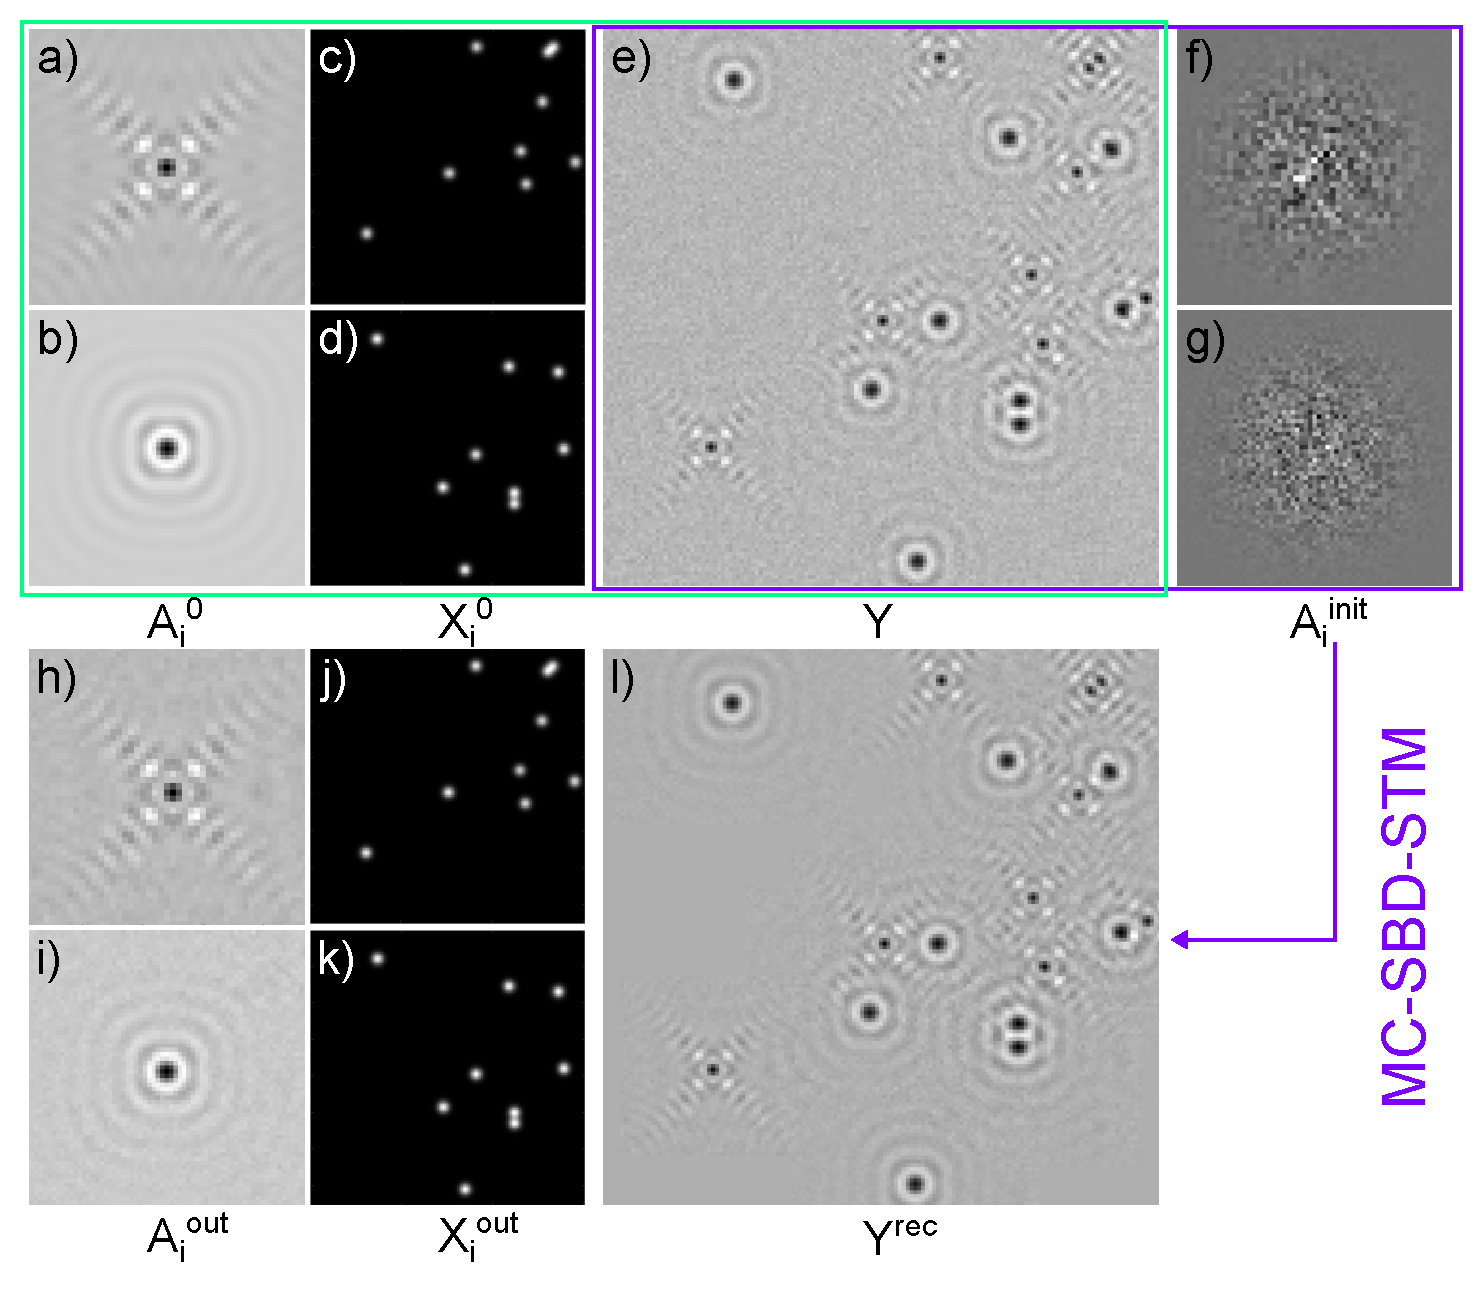
\includegraphics[width= \textwidth]{metric1.pdf} 
	\centering
	\caption[\textbf{An example run of the algorithm on a synthetic dataset}]{\textbf{An example run of the algorithm on a synthetic dataset}. We start from two types of kernels a)-b) and their corresponding activation maps c)-d), and use them to generate the observation $Y$ e). The observation together with two initialized kernels f)-g) are fed into the algorithm, and the resulting kernels and activation maps are shown in h)-k). A reconstructed observation $Y^{rec}$ is plotted in l).}
	\label{fig:metric}
\end{figure}

The algorithm outputs $A_i^{out}$ and $X_i^{out}$. It successfully demixed two types of kernels and reconstructed an observation $Y^{rec}$ that is similar to the original observation $Y$. Note that $Y^{rec} = \sum_i A^{out}_i * X^{out}_i$, not a direct output from the algorithm. Moreover, all the activation maps shown in Fig. \ref{fig:metric} are generated by applying a Gaussian window to the original discrete activation, for reasons that we will elaborate when discussing the Activation Similarity metric. 

Before showing the resulting metric scores for this example run, we first elaborate how each metric is established and what aspects of performance does it evaluate. 
\begin{itemize}
	\item \textbf{Kernel Similarity(\textit{KS})}: 
	\begin{equation}
		\textbf{\textit{KS}} = \frac{\operatorname{FT}(A_i^0)_{\textit{flatten}} \cdot  \operatorname{FT}(A_i^{out})_{\textit{flatten}}}{\vert \vert \operatorname{FT}(A_i^0)_{\textit{flatten}} \vert \vert \cdot  \vert \vert \operatorname{FT}(A_i^{out})_{\textit{flatten}}\vert \vert}
	\end{equation}
	\textbf{\textit{KS}} directly evaluates how well the outcome kernel matches with the ground truth kernel, by calculating the cosine similarity between the ground truth kernels and the output kernels in the q-space. Performing Fourier transform first enforces centering of the \ac{QPI} pattern, thus the cosine similarity is only sensitive to the actual feature of the kernel, but robust against any in-plane shift in the real-space kernel. 
	
	\item \textbf{Activation Similarity(\textit{AS})}: 
	\begin{equation}
		\textbf{\textit{AS}} = \frac{\operatorname{GW}(X_i^0)_{\textit{flatten}} \cdot  \operatorname{GW}(X_i^{out})_{\textit{flatten}}}{\vert \vert \operatorname{GW}(X_i^0)_{\textit{flatten}} \vert \vert \cdot  \vert \vert \operatorname{GW}(X_i^{out})_{\textit{flatten}}\vert \vert}
	\end{equation}
	\textbf{\textit{AS}} evaluates how well the outcome activation map matches with the ground truth activation map, by calculating the cosine similarity between the Gaussian windowed ground truth activation and the Gaussian windowed output activation. The GW is applied to reduce the influence of tiny misalignment while preserving the dominating features of the activation map. This allows us to construct a more continuous and robust metric to evaluate the performance. More specifically, the square GW is defined as: $g(r)= e^{\frac{r^2}{2 \sigma}}$, where $\sigma = \operatorname{min}(\frac{1}{3}\sqrt{\frac{-ln(0.95)}{\rho \pi}}, \frac{\textbf{\textit{kernel size}}}{10})$. $\rho$ is the fraction of active pixels in the activation map, and \textbf{\textit{kernel size}} is the side length of the kernel associated with this activation. This means if activations are sparse (low density), the filter becomes broader to average over a wider area, while if activations are dense, the filter stays sharper.
	
	\item \textbf{Observation fidelity(\textit{OF})}
	\begin{equation}
		\textbf{\textit{OF}} = \operatorname{variance}(noise)/\operatorname{variance}(Y_{residual}),
	\end{equation}
	where $Y_{residual} = Y - Y_{reconstructed} = Y - \sum_i(A^{out}_i * X^{out}_i)$, and $noise$ is the noise term in Equation. \ref{eq:observation}. In an ideal case, where $A^{out}_i = A^{0}_i$ and $X^{out}_i = X^{0}_i$, the discrepancy between $Y_{reconstructed}$ and $Y$ will be at the noise level. Thus, a successful run of the algorithm will give \textbf{\textit{OF}} $\approx$ 1. We can further exemplify this by plotting all observations and noise level under the same color limit as shown in Figure. \ref{fig:OF}, we can see that c) and d) have similar variance. Note that the observation fidelity is the ultimate metric we will use to evaluate the performance of the reconstruction in real data. 
	
	\item \textbf{Demixing Score(\textit{DS})}:
	\begin{align}
		\textbf{\textit{DS}} &= 1 - \operatorname{softIoU}(X_i^{out},X_j^{out}) \\
		&= 1 - \frac{\sum(\operatorname{min}((X_i^{out})_{flatten}, (X_j^{out})_{flatten}))}{\sum(\operatorname{max}((X_i^{out})_{flatten}, (X_j^{out})_{flatten}))}
	\end{align}
	\textbf{\textit{DS}} evaluates how little two activation maps of different kernel types overlap using soften Intersection over Union(softIoU); it computes the ratio between the overlapping region and the union region over two images, with the mathematical form elaborated above. The rational is that the probability of two different types of defects sitting on the same lattice site is near zero; Thus, a successful demixing should give \textbf{\textit{DS}} close to 1. Note that this metric relies solely on the output activation and thus can also be applied to real data.  
\end{itemize}

The scores of the four metrics for this example run are listed in Table 6.1, all of which indicate a successful execution of the algorithm. In particular, we observe a perfect match for the activation maps, as illustrated in Figure \ref{fig:metric} (panels c, d, j, k). Regarding kernel similarities, both \textbf{\textit{KS}} values exceed 0.95, indicating a near-perfect match. To examine this more closely, Figure \ref{fig:KS} presents the detailed \ac{QPI} patterns in both real and reciprocal spaces for type two. From left to right, the three columns show the noiseless ground truth kernel, the output kernel, and the noisy ground truth kernel.

Since the input observation $Y$ is noisy, it would be natural to expect the output kernel to resemble the noisy ground truth kernel. However, the output kernel actually captures more structural information than the noisy ground truth, as evident in the reciprocal \ac{QPI} patterns. For example, panel e shows faint square arcs outside the high-intensity diamond features, which also faintly appear in panel d but are entirely absent in panel f. This is a surprising, yet consistent, outcome across multiple datasets.

The reason is that while the noise is random, the algorithm identifies repetitive units (the kernels) throughout the entire observation, and the signals from all activation sites are taken into account. As a result, the reconstructed kernel is effectively an average over all the instances. It is thus denoised and resembles the noiseless ground truth more closely than the noisy input. This highlights the advantages of this novel approach compared to conventional methods like simple cropping.

Nevertheless, despite this denoising effect, the output kernel still retains some random fluctuations, which makes a perfect match with the noiseless ground truth impossible. In fact, these random fluctuations are exploited by the algorithm to further reduce the residual, contributing to the overfitting factor of $\textbf{\textit{OF}} = 1.34 > 1 $, This elevated \textbf{\textit{OF}} suggests mild overfitting, likely driven by those same random fluctuations in the reconstructed kernel. A detailed comparison between $Y^{res}$ and $Noise$ is provided in Figure. \ref{fig:OF}
% todo: can make a plot of all averaged vs out kernel.  

\begin{table}[h]
	\label{table:metric}
	\centering
	\begin{tabular}{|l|c|c|}
		\hline
		\textbf{Metric} & \textbf{Kernel 1} & \textbf{Kernel 2} \\
		\hline
		Kernel Similarity & 0.9749 & 0.9701 \\
		\hline
		Activation Similarity & 0.9983 & 0.9994 \\
		\hline
		Separation Score & \multicolumn{2}{c|}{0.9999} \\
		\hline
		Observation Fidelity & \multicolumn{2}{c|}{1.34} \\
		\hline
	\end{tabular}
	\caption{Quantitative evaluation of kernel and activation similarity, separation, and observation fidelity for two kernel types.}
\end{table}

\begin{figure}
	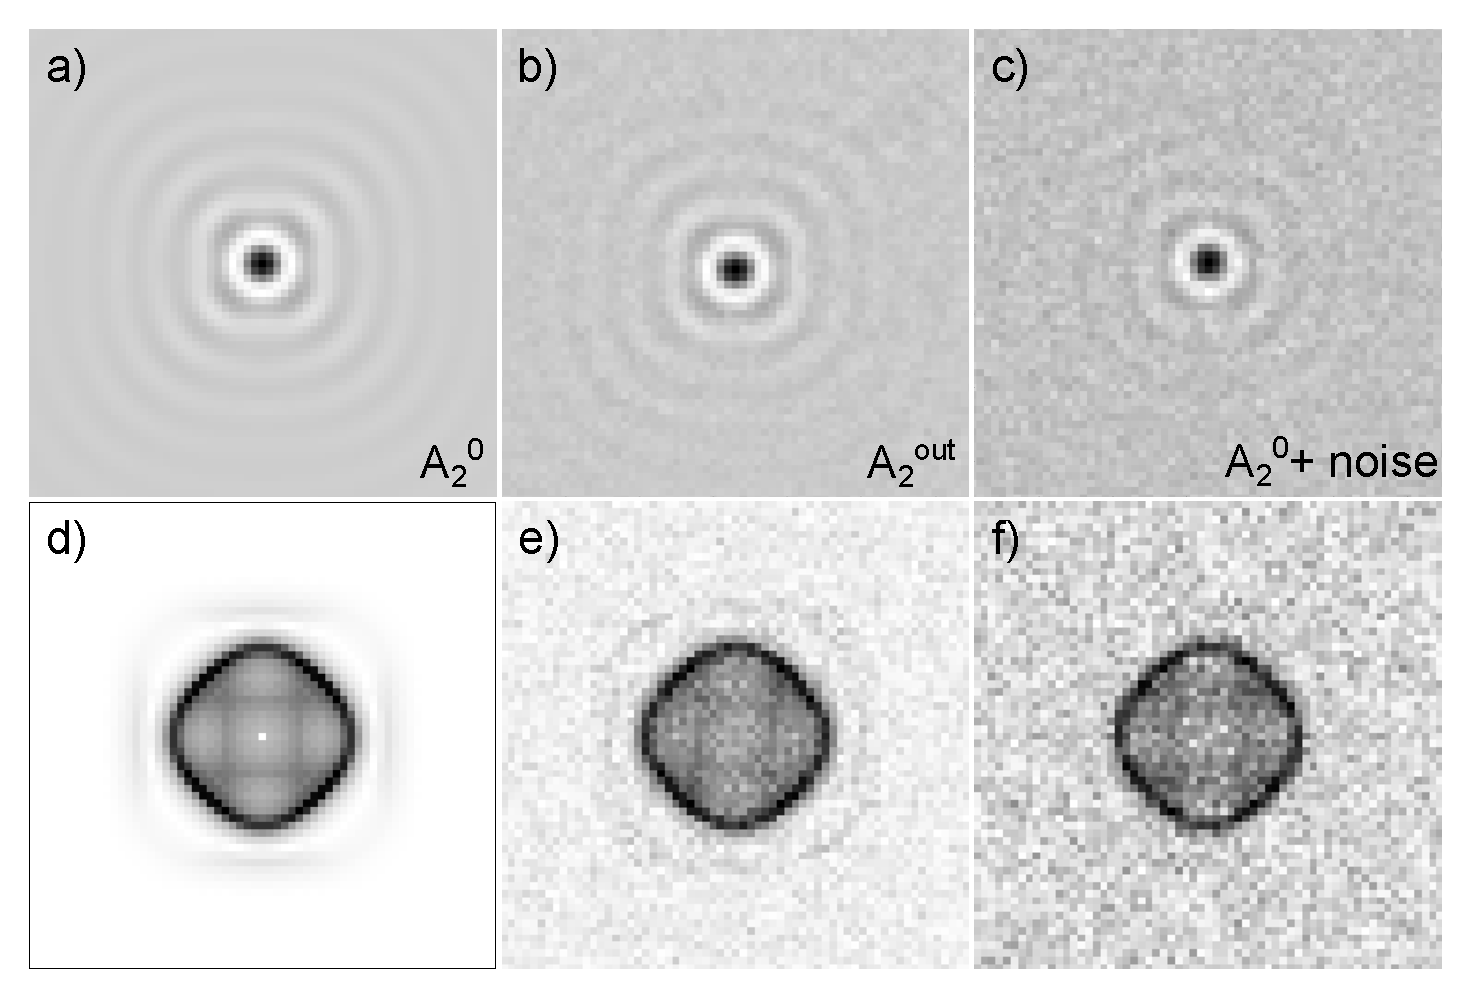
\includegraphics[width= \textwidth]{KS.pdf} 
	\centering
	\caption[\textbf{Comparison between the output kernel and ground truth kernels}]{\textbf{Comparison between the output kernel and ground truth kernels}. a)-c): noiseless ground truth kernel $A_2^0$, output kernel $A_2^{out}$ and ground truth kernel plus noise on the same level as the observation. d)-f): the Fourier transformed q-space kernels, we can see that the output kernel d) recovers the outermost arc feature that are presented in the noiseless ground truth kernel e), but not in f).}
	\label{fig:KS}
\end{figure}

\begin{figure}
	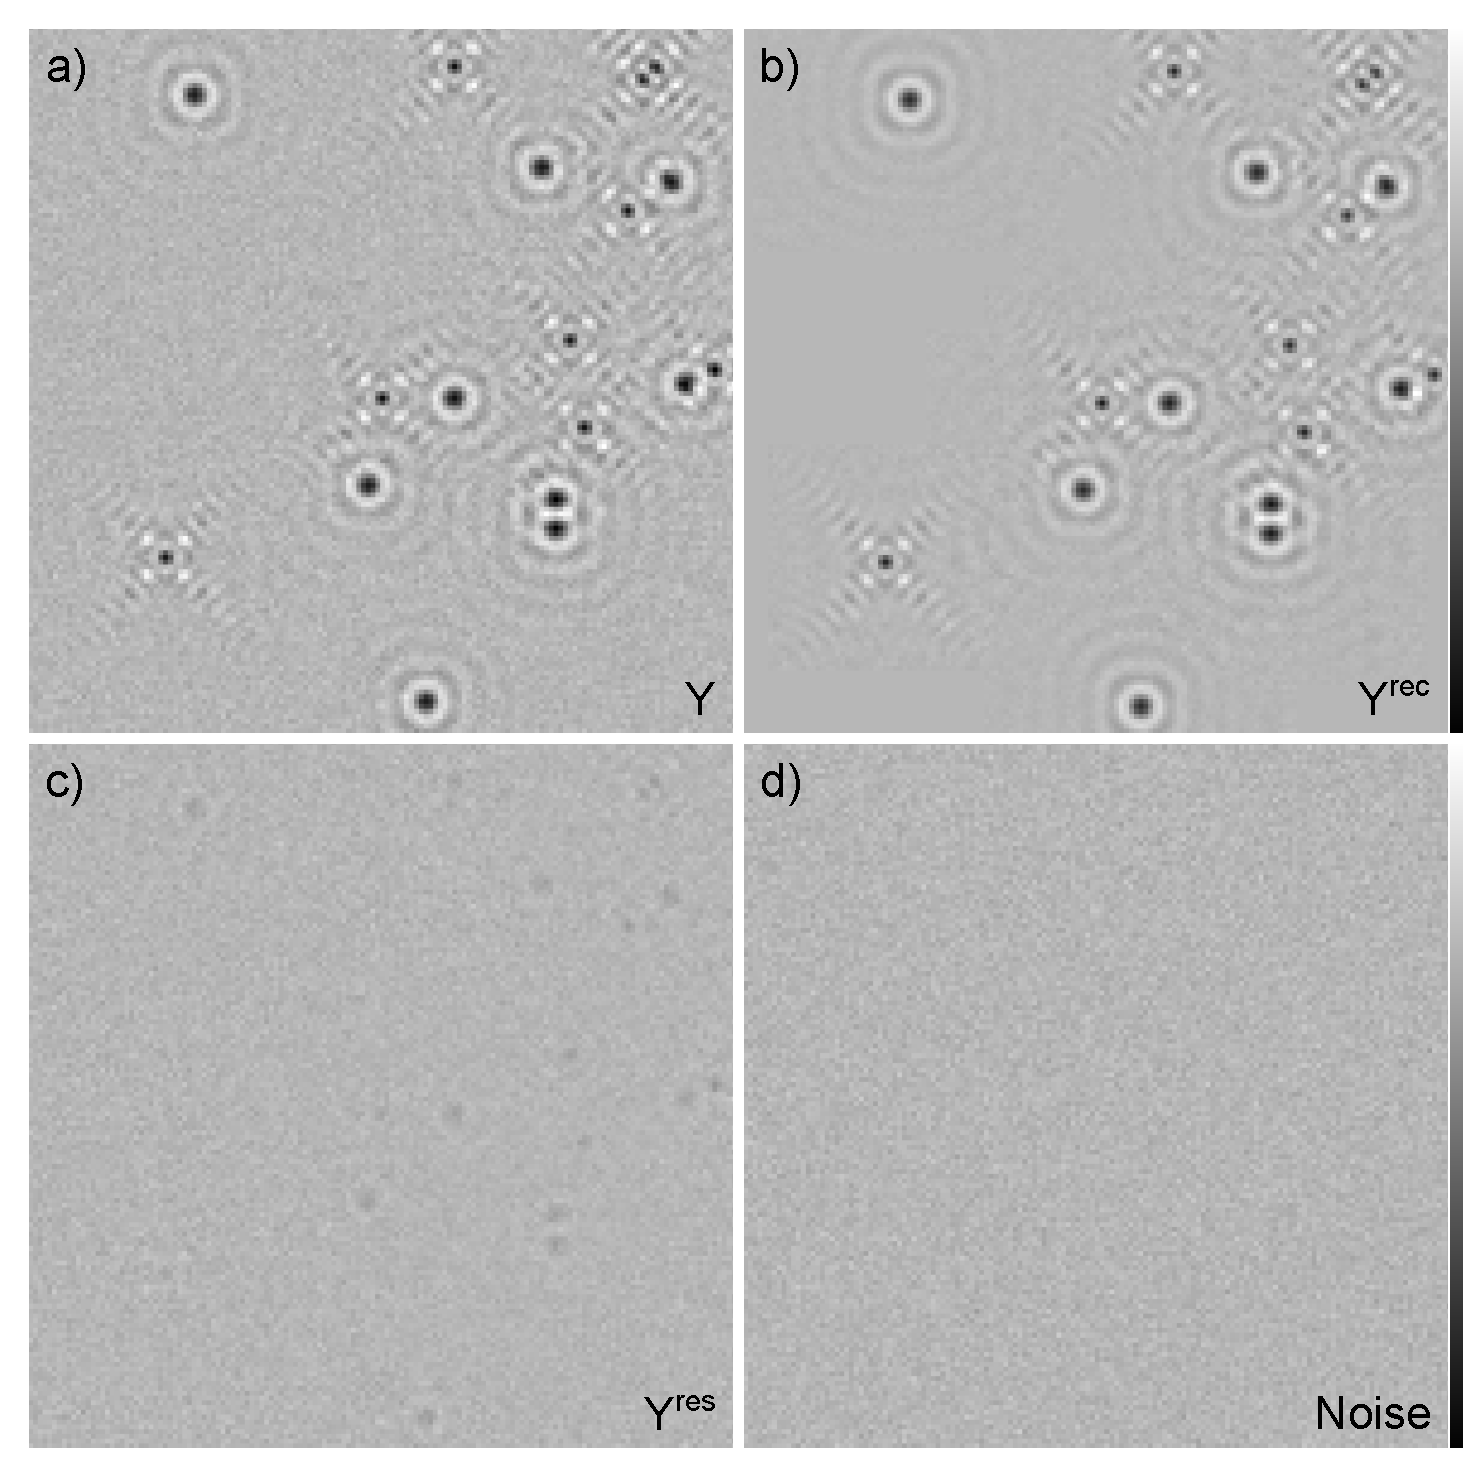
\includegraphics[width= \textwidth]{OF.pdf} 
	\centering
	\caption[\textbf{Illustration of the observation fidelity(OF)}]{\textbf{Illustration of the observation fidelity(OF)}. \textbf{\textit{OF}} quantifies how close the residual observation $Y^{res}$ in c) is to the noise in d). Where $Y^{res}$ is the difference between the reconstructed observation $Y^{rec}$ and input observation $Y$.}
	\label{fig:OF}
\end{figure}


\section{Benchmark tests on the dataset parameter space}
Now that we understand what the algorithm can achieve and how to evaluate its performance, it is time to address under what conditions it performs well. Analogous to evaluating an output $y$ given $f(x)=y$, where one must consider both the system parameter space defining the function $f$ and the input parameter space determining $x$, we must consider two aspects of our problem. First, the algorithm itself involves several free parameters, such as the number of decomposition iterations, the sparsity regularizer $\lambda$, and the faint factor $\beta$. We have explored this system parameter space and identified sets of optimal values, the details of which will be provided in the supplementary material.

This section focuses on the second aspect: the dataset parameter space, which governs the input observations. This analysis addresses how broad the input landscape can be while still yielding reliable algorithmic performance, and, in the context of experimental data, what types of measurements are most likely to produce successful outcomes. This, in turn, provides potential guidelines for experimental data acquisition, ensuring the disentanglement of different \ac{QPI} contributions from various defects.

To this end, we generate physics-informed synthetic data with varying parameters and test our algorithm across a range of dataset regimes. Recall that we can explore datasets in these 4 axes: 
\begin{itemize}
	\item 1. noise level - $SNR$, 
	\item 2. Range of the grid map - $N_{obs}$, 
	\item 3. defect density for each type - $\rho_i$,
	\item 4. Spatial resolution of the grid map - $p$.
\end{itemize}
Since it is a common practice to set the spatial resolution as either 2 or 3 when taking a grid map, we will not explore this axis and set $p=3$ for all our datasets. 

Apart from the above parameters, we also tuned the number of different types of defects(or kernel types). However, due to the drastic increase in computational expense with increasing kernel types, we first run a full exploration of the parameter spaces and discuss the results with 2 types of kernels, then we will show result on a toy run with kernel types = 3. 

In the full exploration runs we ran on 2 types of kernels, we run the algorithm on 3 trials with different datasets. The datasets with different parameter sets are listed in Table.6.2. In total, 180 different observations are generated to cover defect density from sparse to dense, grid maps of sizes ranging from $10^2$ to $10^4$ nanometer squares (given a normal bond length is around 2-5 angstrom), and signal to noise ratio from as low as 0.5 to 3. We then collect the results from all the trials and plot the corresponding metrics to a 3D phase space plot shown in Figure. \ref{fig:phase_space}. There are two things to evaluate, the kernel and activation maps, since they can behave differently within the parameter space, we make one subplot each. On the left, we use \textbf{\textit{KS}} to evaluate the performance on the kernel recovery, and on the right, since there are two metrics defined to evaluate the activation maps, for convenience, we use \textbf{Activation map score(\textit{AMS})}:   
\begin{equation}
	\textbf{\textit{AMS}} = \sqrt{\textbf{\textit{AS}} \cdot \textbf{\textit{DS}}}.
\end{equation} 

\begin{table}[h!]
	\label{table: parameter_space}
	\centering
	\begin{tabular}{|l|c|c|c|}
		\hline
		\textbf{Trial} & \textbf{Defect Density} & \textbf{N\_obs} & \textbf{SNR} \\
		\hline
		1 & $[1.0e{-3},\ 1.8e{-3},\ 3.2e{-3},\ 5.6e{-3},\ 1.0e{-2}]$ & $[50,\ 100,\ 150,\ 200]$ & $[1,\ 3,\ 5]$ \\
		2 & $[1.0e{-3},\ 2.4e{-3},\ 5.6e{-3},\ 1.3e{-2},\ 3.2e{-2}]$ & $[50,\ 100,\ 150,\ 200]$ & $[1,\ 2,\ 3]$ \\
		3 & $[1.0e{-3},\ 3.2e{-3},\ 1.0e{-2},\ 3.2e{-2},\ 1.0e{-1}]$ & $[50,\ 100,\ 150,\ 200]$ & $[0.5,\ 1,\ 3]$ \\
		\hline
	\end{tabular}
	\caption{Parameter spaces for the 3 runs. In total 180 datasets where generated to explore 3 axes of parameters.}
\end{table}

\begin{figure}
	\centering
	\makebox[\textwidth][c]{%
		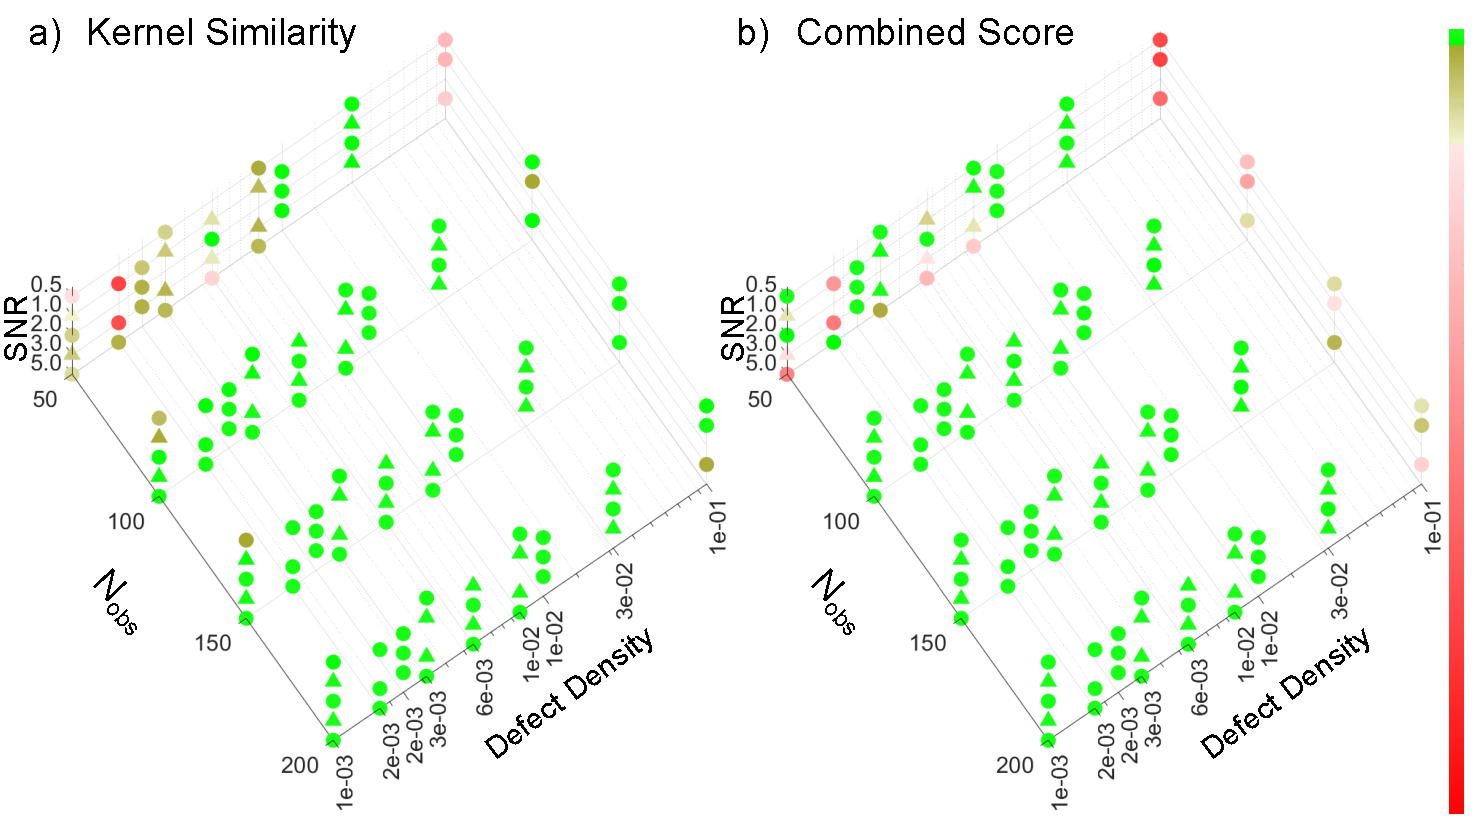
\includegraphics[width=1.5\textwidth]{total_metric_space.pdf}
		}
	\caption[\textbf{Performance metrics on 3D dataset parameter space(Two defect types)}]{\textbf{Performance metrics on 3D dataset parameter space(Two defect types)}. Observations with different dataset parameters are generated and fed into the algorithm, each marker indicates one (circular) or several datasets (triangular). The outputs are evaluated with a) kernel similarity and b) activation combined score, if there are multiple datasets then we take the corresponding average. A colorbar is setup to indicate 3 levels of performance: Red $(0,0.85]$ - failed, Yellow $(0.85,0.98)$ - worked, Green $[0.98,1.00]$ - perfect.}
	\label{fig:phase_space}
\end{figure}

Each marker on the 3D plot represents a single dataset generated in our experiments. As shown in Table.6.2, some datasets share the same initialization parameters; however, because the activation maps are generated randomly, these datasets are not identical. For parameter combinations that occur more than once, the metric value displayed at that point is the average of the metrics from all corresponding datasets. In total, there are 180 datasets exploring 132 different combinations of parameters shown in the plot. A triangular marker indicates an overlapping case, where multiple datasets sharing the same parameter combination, and we take the average of the corresponding metrics; whereas a circular marker indicates a non-overlapping case. The color of each marker indicates the average value of metrics computed over both kernel types within each individual dataset. The metric colorbar of two subplots is defined in the same way; It has 3 sections, red section ranging from $[0.0, 0.85]$, yellow section from $[0.85,0.98]$, and the green section for metrics within $[0.98,1]$. The colorbar is designed around 2 thresholds that are empirically chosen based on manual observation. $0.85$ is the pass line for a given recovery, below which the recovery is considered failed. Values above $0.98$ give recoveries that are indistinguishable from the ground-truth kernels and activation maps, and thus are considered a success. It is also worth noting that the ground-truth kernels used in \textbf{\textit{KS}} calculations are noiseless ground-truth, like panel a) in Figure. \ref{fig:KS}. This sets an even higher standard for the algorithm. 

\begin{figure}
	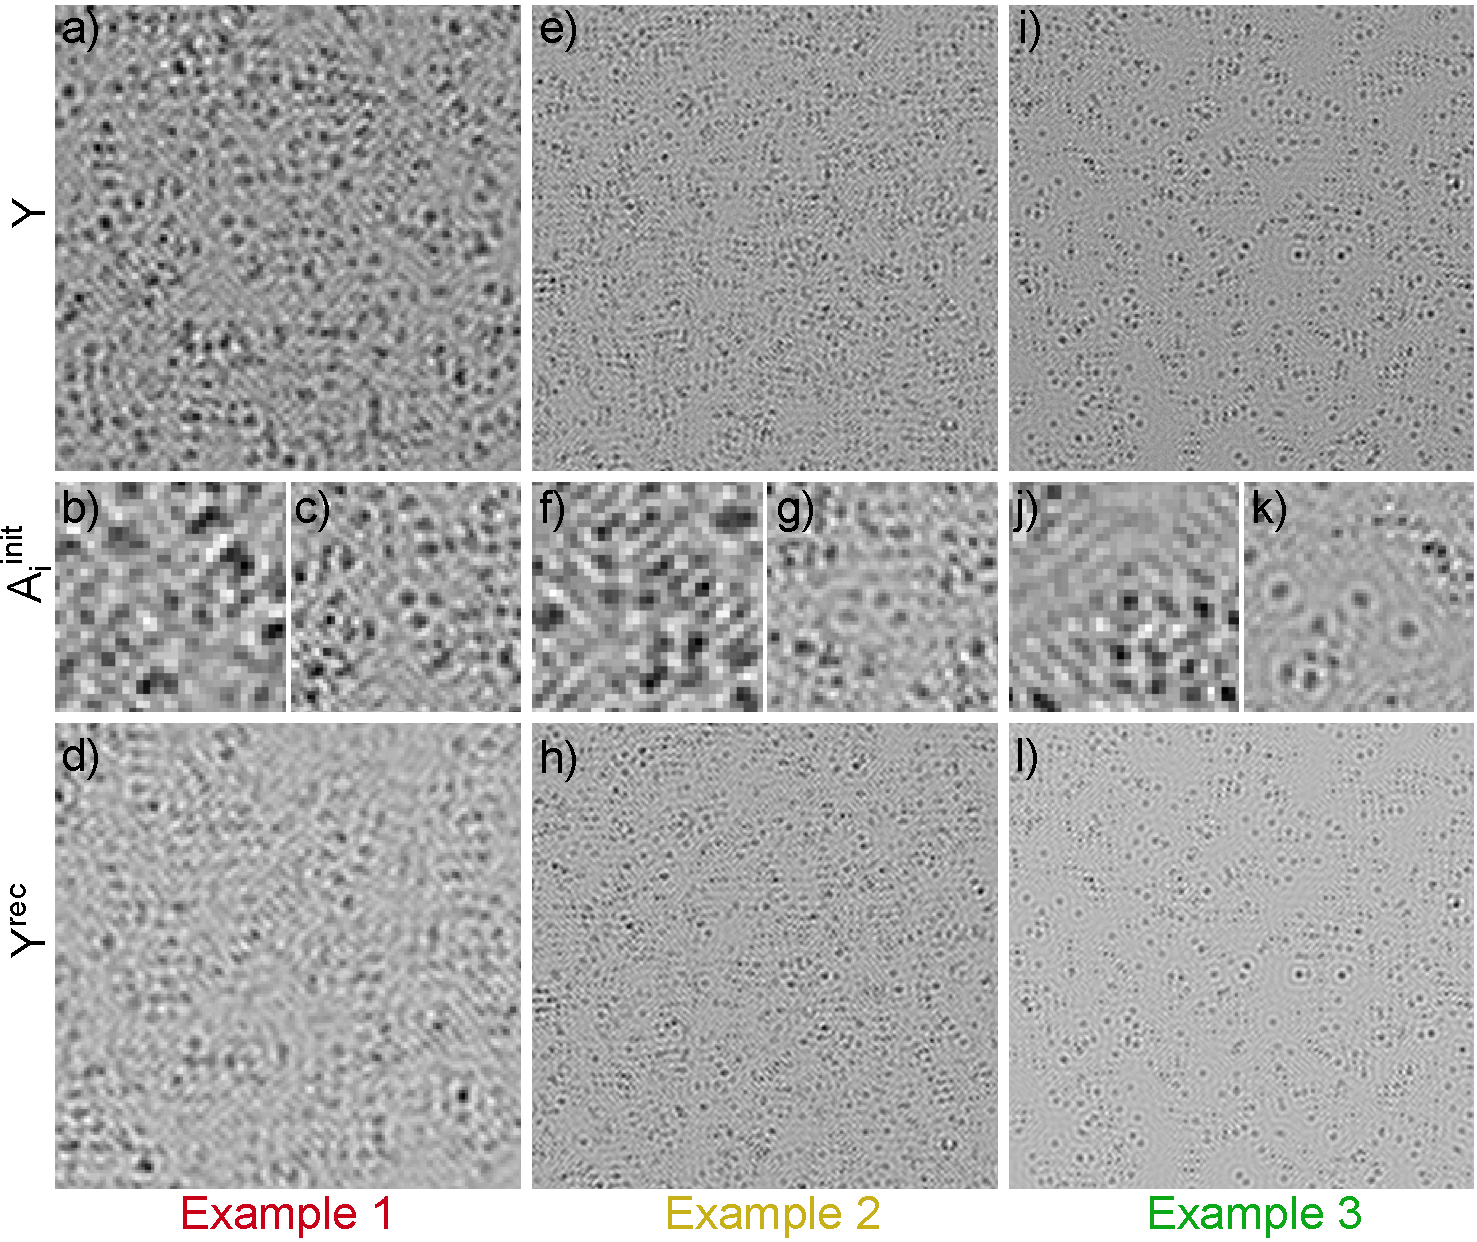
\includegraphics[width= \textwidth]{3trials.pdf} 
	\centering
	\caption[\textbf{Initialization and reconstruction results of three examples}]{\textbf{Initialization and reconstruction results of three examples}. Three examples are arranged column-wise, and the three rows represents the observation $Y$, initialized kernels $A^{init}$ and the reconstructed observations $Y{rec}$, respectively. a): observation generated from $N_{obs} = 50$, $\rho_i = 1e-1$, $SNR = 1$, e): observation generated from $N_{obs} = 100$, $\rho_i = 1e-1$, $SNR = 1$, i): observation generated from $N_{obs} = 100$, $\rho_i = 3e-2$, $SNR = 1$. The initialized kernels (b-c, f-g, j-k) are generated by cropping around an existing ground truth activation point of that kernel type. The reconstructed observations (d, h, l) are the convolution of corresponding output kernels and activation maps.}
	\label{fig:regimes}
\end{figure}

To help establishing some intuitions behind the reconstruction quality in different regimes, we will elaborate three examples selected from the red, yellow and green regime of Figure. \ref{fig:phase_space}, respectively. More specifically, the parameter combinations are: 
\begin{itemize}
	\item Example 1(Red regime): $N_{obs} = 50$, $\rho_i = 1e-1$, $SNR = 1$;
	\item Example 2(Yellow regime): $N_{obs} = 100$, $\rho_i = 1e-1$, $SNR = 1$;
	\item Example 3(Green regime): $N_{obs} = 100$, $\rho_i = 3e-2$, $SNR = 1$;
\end{itemize}

We show the initialization and reconstructions of these 3 runs in Figure. \ref{fig:regimes}, and present their detailed output kernels in Figure. \ref{fig:regimes_closer}. Note that all the initialized kernels in second row of Figure. \ref{fig:regimes} are obtained by cropping around a ground truth activation point of that kernel type. Due to the dense defect concentrations, it is difficult to tell from the $Y^{rec}$ whether the reconstructions are successful; it is less dense for example 3, and we can see $Y^{rec}$ matches perfectly with $Y$. We then take a closer look into the output kernel qualities in each example in Figure. \ref{fig:regimes_closer}, where the output kernels $A_1^{out}$, $A_2^{out}$ and their associated Fourier transforms of each example are presented column-wise. The last column shows the ground truth for better comparison. For example 1, features in a) and i) are completely different from the ground truth; both output kernel has kernel similarity score of around 0.65; this indicates the failing of the algorithm. On the contrary, example 3 present a perfect match compared to the ground truth, in both the real space and q-space. This empirical observation matches the metric scores of close to unity for both kernels. Example 2 outputs kernels that are less ideal, and give metrics landing in the yellow regime; while the overall features of both kernels match that of the ground truth, clear discrepancies exist. More specifically, a mixture of features in b) and j) are observed. We can see this leakage better in q-space, note the ground truth kernel 1 h) and kernel 2 p) are featured with these 4 arcs (with highest intensity) and the rounded diamond (with highest intensity), respectively. However, the 4 arcs that belong to ground truth kernel 1 is also found in the n), the output kernel 2 in example 2; and the rounded diamond feature is found in f). The root cause of the mixture of features is linked back to the associative symmetry of multi-channel convolution as discussed in Chapter 5.2, and this shows that this dataset setting is pushing the performance limit of this algorithm.

\begin{figure}
	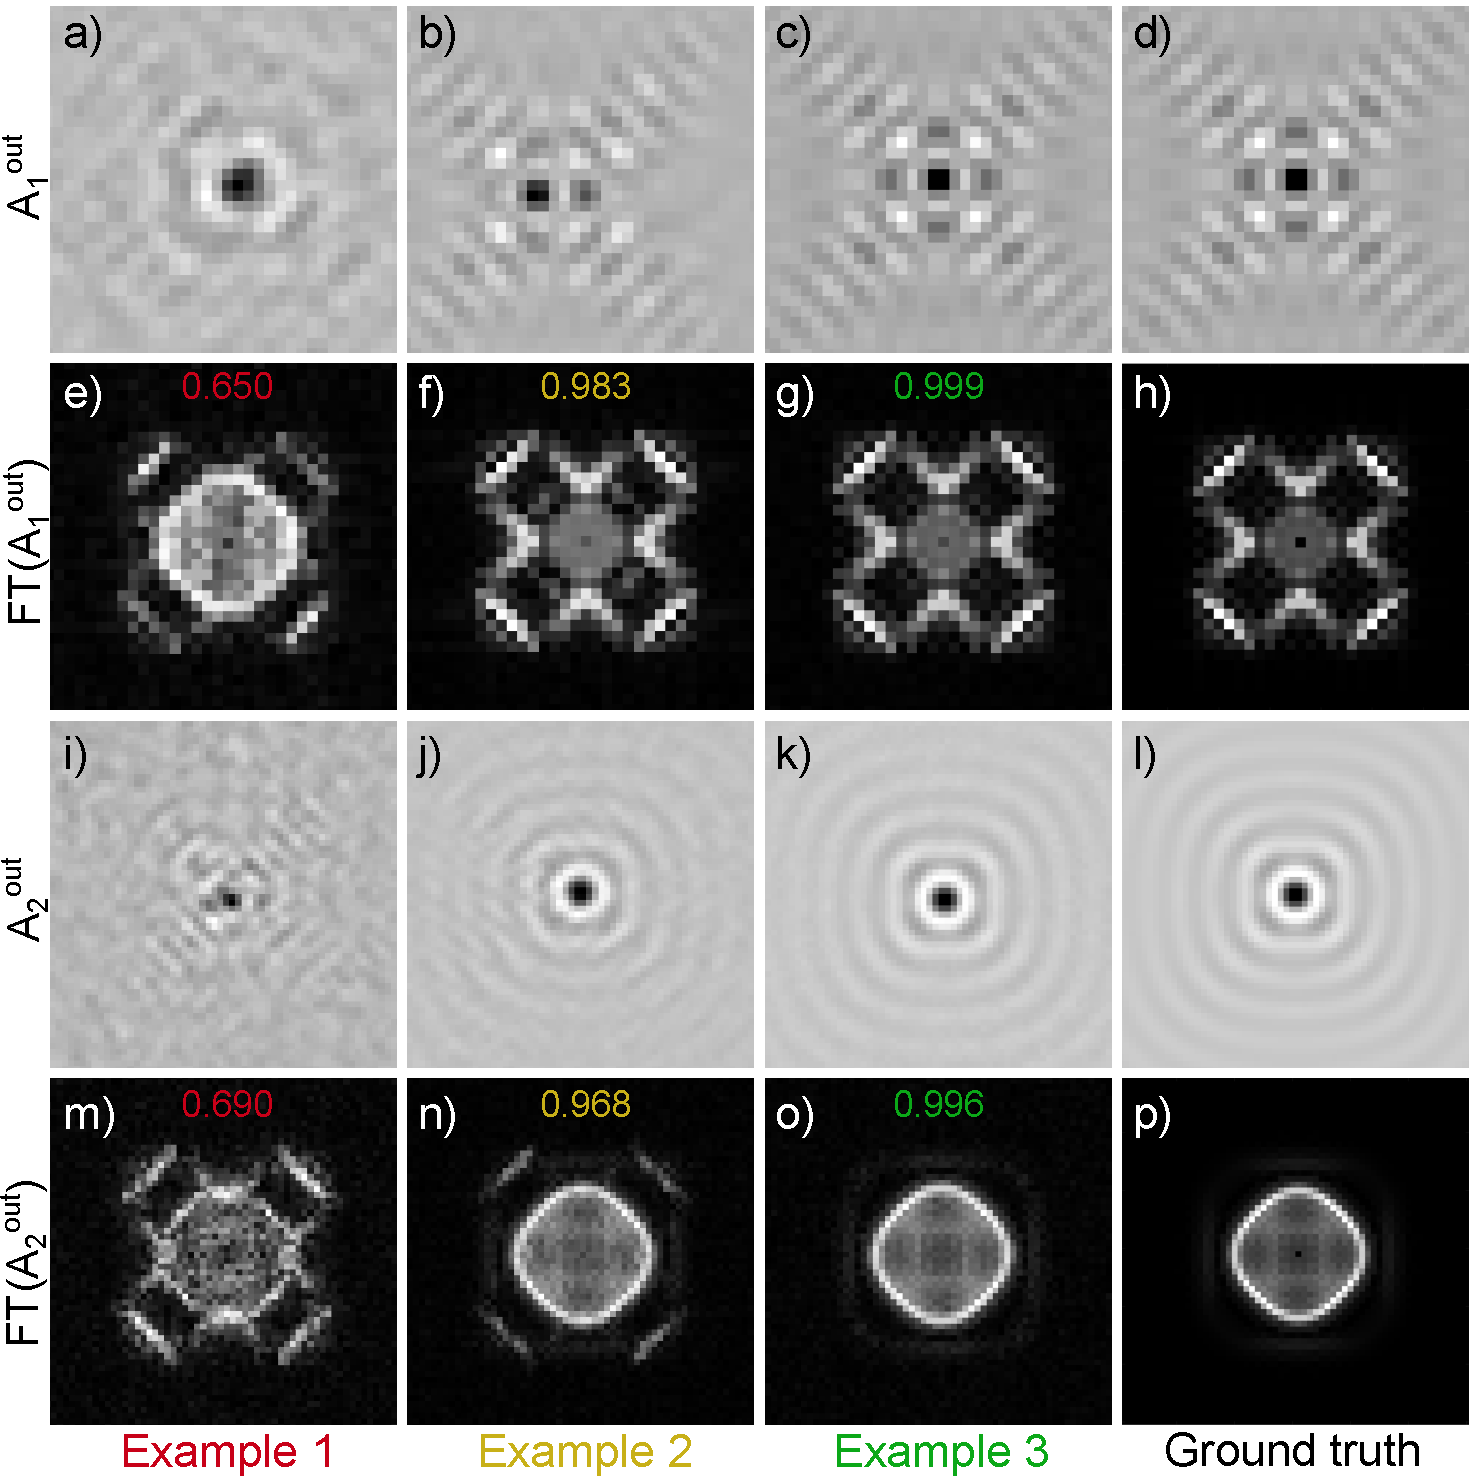
\includegraphics[width= \textwidth]{3trials_closer.pdf} 
	\centering
	\caption[\textbf{Output kernel quality illustration for three examples}]{\textbf{Output kernel quality illustration for three examples}. a)-c) are the real space output kernels for three examples. We then Fourier transform these real space kernels to q-space and get e)-g), each Fourier transformed image has a number attached showing its kernel similarity score. i)-k) and m)-o) are the repetition for kernel 2. For better comparison, the last column of images show the ground truth kernels and their Fourier transform. We can see that example 1 completely failed the reconstruction, example 3 has a perfect kernel reconstruction, and example 2 shows output kernels similar to the ground truth, but it also has some discrepancies to the ground truth that could be easily spotted in f) and n).}
	\label{fig:regimes_closer}
\end{figure}

We also performed a similar phase space experiment for datasets with 3 defect types, and the result is shown in \ref{fig:phase_spaceN=3}. Despite that the phase space consists less data points, it gives similar trend as the 2-defect-type case. The algorithm failed on extremely high defect density cases, and generate output with worse quality with increasing noise level and decreasing $N_{obs}$ 

\begin{figure}
	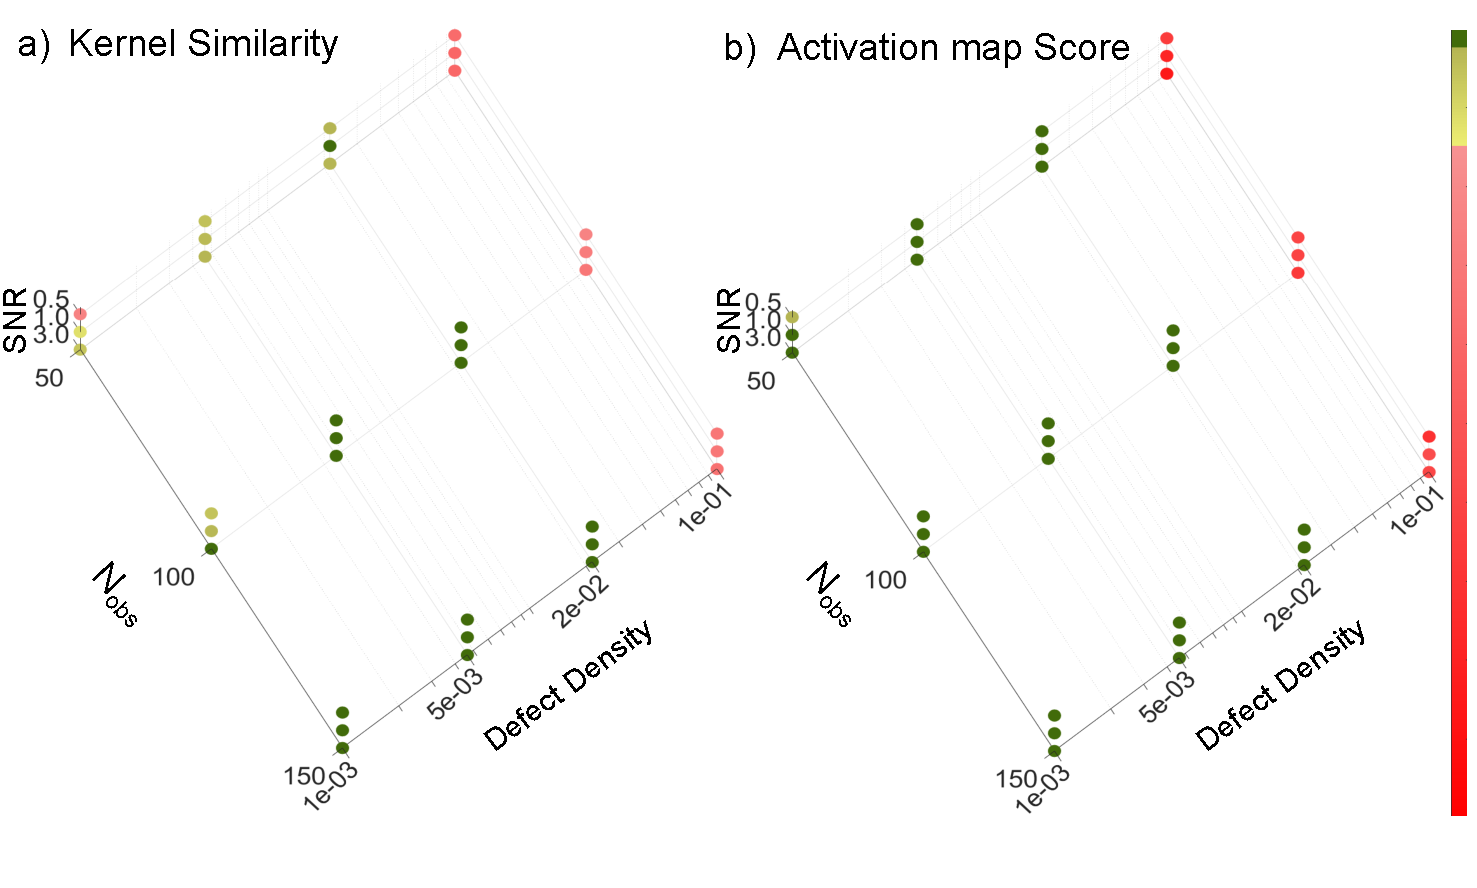
\includegraphics[width= \textwidth]{phase_space_3kernel.pdf} 
	\centering
	\caption[\textbf{Performance metrics on 3D dataset parameter space(Three defect types)}]{\textbf{Performance metrics on 3D dataset parameter space(Three defect types)}, Observations with different dataset parameters are generated and fed into the algorithm, each marker indicates result from one dataset generated by the corresponding dataset parameters. The outputs are evaluated with a) kernel similarity and b) activation combined score. A colorbar is setup to indicate 3 levels of performance: Red $(0,0.85]$ - failed, Yellow $(0.85,0.98)$ - worked, Green $[0.98,1.00]$ - perfect. Result from this three defect types experiments possess similar qualitative trend as of the 2-defect-type case.}
	\label{fig:phase_spaceN=3}
\end{figure}
\subsection{discussion on the phase space}
In general, the algorithm works in most of the phase space we explore. More specifically, it is very successful on datasets with low to medium defect concentration, medium to big $N_{obs}$, and higher SNR. This give us a reference on the robustness of this algorithm, and a rough estimate on the algorithm's effectiveness on real data within these regimes.

\begin{figure}
	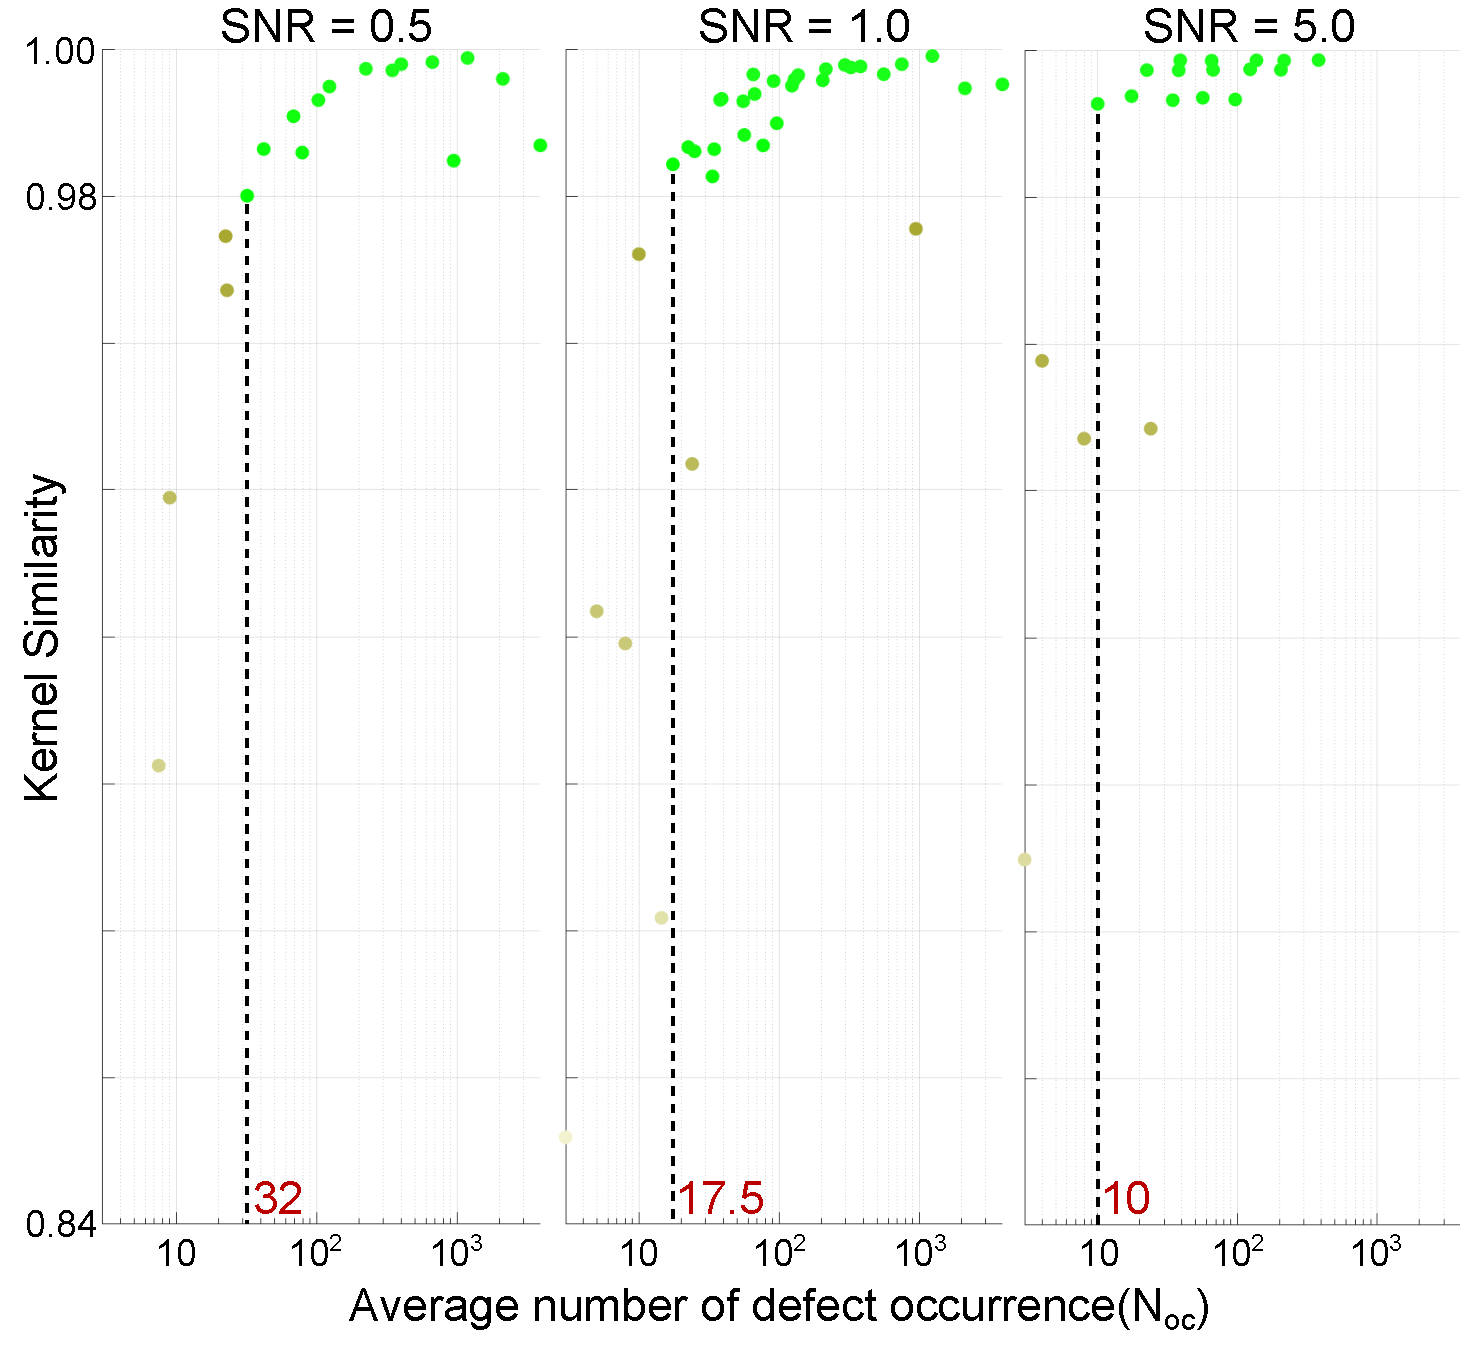
\includegraphics[width= \textwidth]{KS_vs_N.pdf} 
	\centering
	\caption[\textbf{Relationship between the average number of defect occurrences and kernel similarity}]{\textbf{Relationship between the average number of defect occurrences and kernel similarity} For a): $SNR=0.5$, b): $SNR=3$, c): $SNR=5$. Each point represents a dataset on the metric phase space, with $N_{oc} = \rho_i * N_{obs}^2$. A clear positive correlation is observed: as the number of defect occurrences increases, kernel similarity improves due to stronger denoising effects. The first data point exceeding a similarity of 0.98 is marked, defining a critical occurrence threshold $N^{critical}$, below which reconstruction quality degrades. Higher $SNR$ values reduce the required $N^{critical}$, consistent with the intuition that less noisy kernels require fewer samples for accurate reconstruction.}
	\label{fig:KS_vs_N}
\end{figure}

We also observe that the two metrics we used respond differently with different parameters. Kernel similarity is more sensitive to the size of scans, with smaller scan sizes, for example when $N_{obs} = 50$, the kernel reconstruction works less well. This is likely because of the denoising effect that we discussed; At fixed defect density, the number of occurrence of each kernel drops as we decrease $N_{obs}$, this weakens the denoising effect and makes the output kernels more noisy and less similar to the noiseless ground truth kernels. This effect can be better seen with Figure. \ref{fig:KS_vs_N}, where we plot the average number of defect occurrence versus the kernel similarity. We see a clear trend that as the occurrence increases, we generally have a better kernel reconstruction. Moreover, we can mark the first data point whose kernel similarity exceeds 0.98, its defect occurrence act as a threshold, below which the reconstruction becomes less optimal. We see that as the $SNR$ increases, the critical defect occurrence $N^{\text{critical}}$ decreases; this observation matches our understanding that in a successful reconstruction, the output kernel is essentially the average of the noisy ground truth kernel, and if $A^0_{\text{noisy}}$ is less noisy to begin with, we need fewer instances to get a desired kernel similarity.   

By observing the activation combined score, we see that the algorithm breaks down at extremely high defect concentration. It is worth noting that $\rho_i = 10\%$ is chosen to test the limit of the algorithm, and the corresponding observation looks something like Figure. \ref{fig:edge_case} a), an observation generated with parameters: $\rho_i = 10\%$, $N_{obs}=100$, $SNR=3$. Despite the extreme difficulty, the algorithm still works and is able to demix and deconvolute kernels with high kernel similarity, as shown in c) and d). The high defect density makes the initial observation full of interference between different kernels; this greatly increases the difficulty in demixing different types of defects, and causes problem of feature leakage as shown in example 2 of Figure. \ref{fig:regimes_closer}.  


To conclude, kernel similarity is more sensitive to the number of defect occurrences, while the activation map score is more closely correlated with defect density. This distinction reflects two core mechanisms of the algorithm: the denoising capability relies on averaging multiple instances of defect-induced QPI signals, whereas the demixing capability deteriorates when interference between patterns from different defect types increases. These insights reveal the limits of the algorithm under challenging conditions.

Nonetheless, by performing benchmark tests across a broad dataset parameter space and evaluating both kernel and activation metrics, we find that the algorithm performs exceptionally well under a wide range of conditions. This demonstrates its robustness and reliability, particularly when datasets provide sufficient coverage and quality. With this confidence established through synthetic testing, we now turn to applying the algorithm to real experimental data.

\begin{figure}
	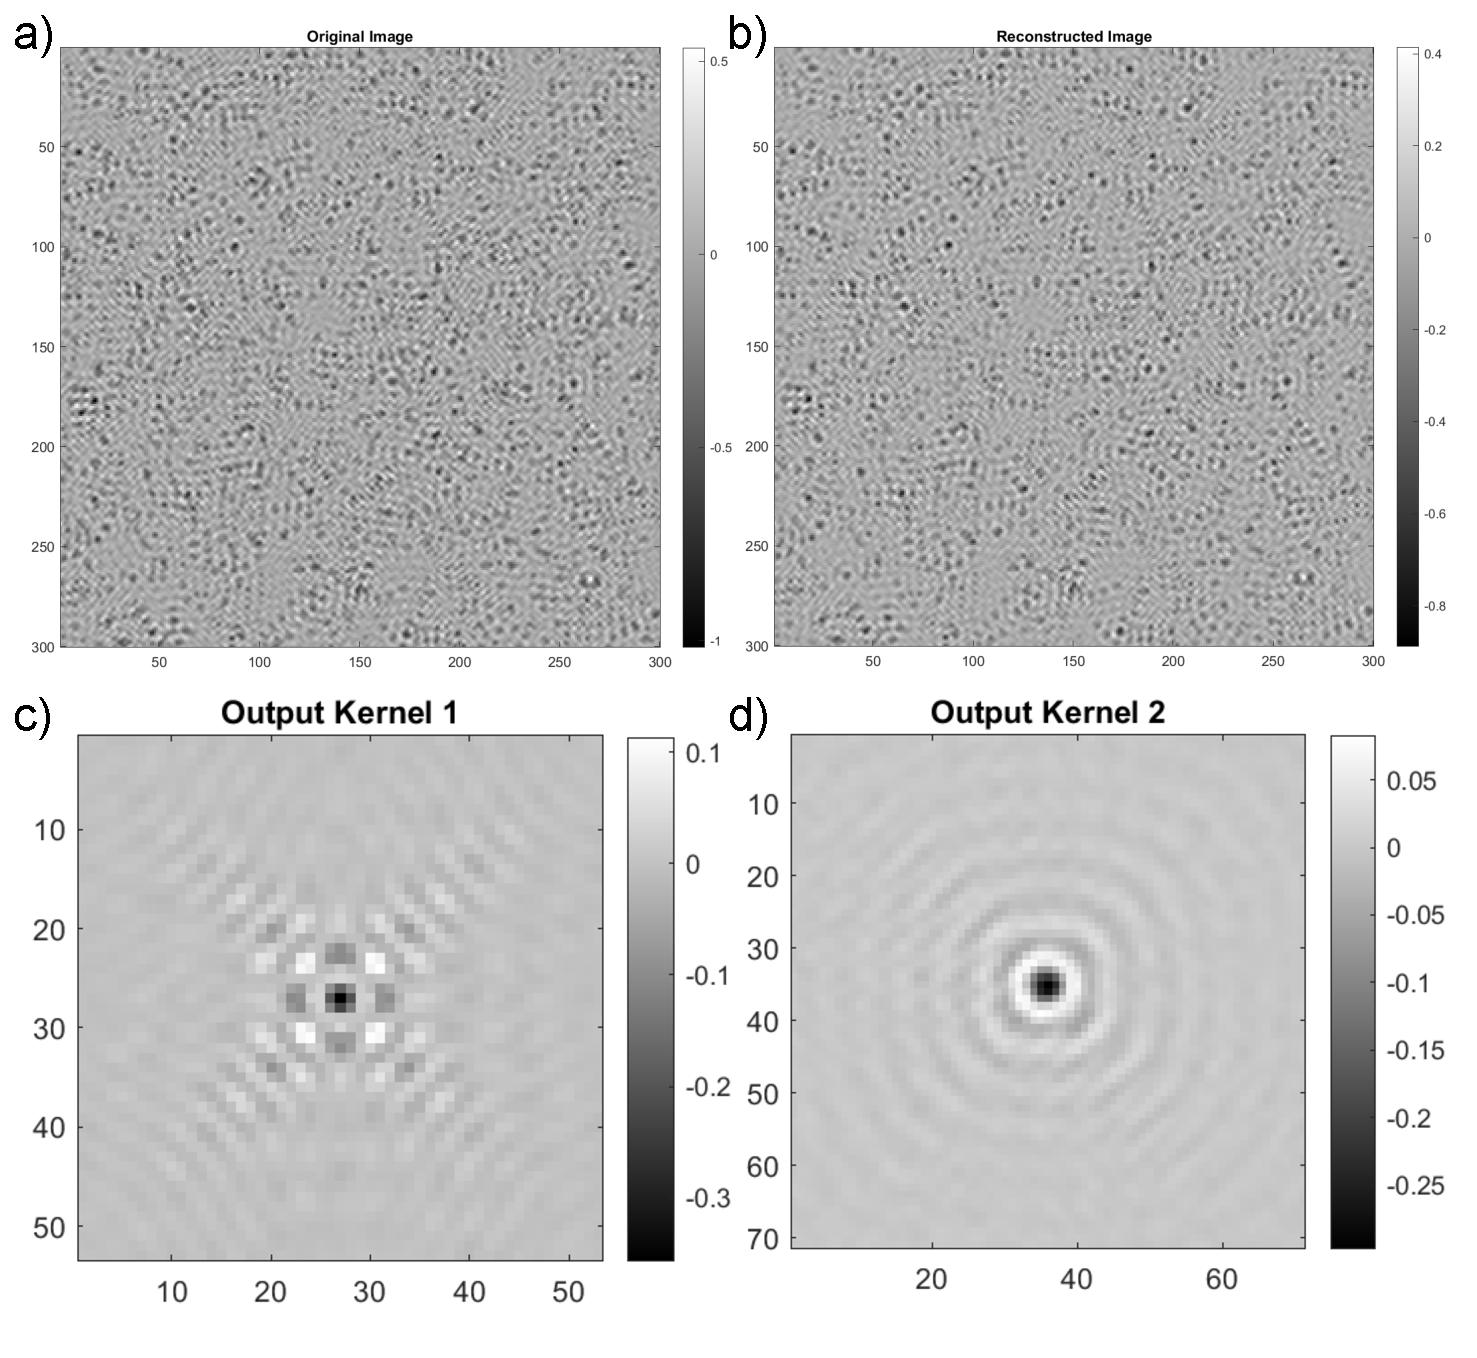
\includegraphics[width= \textwidth]{edge_case.pdf} 
	\centering
	\caption[\textbf{An edge case with extreme defect concentration}]{\textbf{An edge case with extreme defect concentration}. a) observation generated with $\rho_i = 10\%$, $N_{obs}=100$, $SNR=3$, b) reconstructed observation from the algorithm c)-d): output kernels.}
	\label{fig:edge_case}
\end{figure}

